\documentclass[a4paper, 12pt]{article}

% Layout
\usepackage{geometry}
\geometry{left=20mm}
\geometry{right=15mm}
\geometry{top=20mm}
\geometry{bottom=20mm}

% Paragraph
\usepackage{indentfirst}
\setlength{\parindent}{0.75cm}
\linespread{1.25}

% Font
\usepackage{fontspec}
\usepackage[english,russian]{babel}
\usepackage{microtype}

% \usepackage{polyglossia}
% \setmainlanguage{russian}
% \setotherlanguage{english}

% \newfontfamily{\cyrillicfont}{Droid Serif}
% \newfontfamily{\cyrillicfontrm}{Droid Serif}
% \newfontfamily{\cyrillicfontsf}{Droid Sans}
% \newfontfamily{\cyrillicfonttt}{DejaVu Sans Mono}

\setmainfont{Droid Serif}
\setromanfont{Droid Serif}
\setsansfont{Droid Sans}
\setmonofont{DejaVu Sans Mono}

% Hyphens
\usepackage{hyphenat}
\usepackage{ucharclasses}
\setTransitionsForLatin{\begingroup\hyphenrules{english}}{\endgroup}

% Formulas
\usepackage{amssymb, amsfonts, amsmath}

% Miscellaneous
\usepackage{enumerate}
\usepackage{float}
\usepackage{multirow}

% Hyper references
\usepackage{hyperref}
\hypersetup{
    hidelinks,
    allcolors=black
}

% Images
\usepackage{graphicx}
\graphicspath{ {images/} }

%Including title
\usepackage{pdfpages}

% Figures
\usepackage{chngcntr}
\counterwithin{figure}{section}
\usepackage{subcaption}
\renewcommand\thesubfigure{\asbuk{subfigure})}
\captionsetup[subfigure]{labelformat=simple, labelsep=space}

% Counters
\usepackage[figure,table,page]{totalcount}
\usepackage{totcount}

% Code listings
\usepackage{listings}
\usepackage{xcolor}

\definecolor{codegreen}{rgb}{0,0.6,0}
\definecolor{codepurple}{rgb}{0.58,0,0.82}
\lstdefinestyle{codestyle}{
    commentstyle=\color{codegreen},
    keywordstyle=\color{magenta},
    stringstyle=\color{codepurple},
    basicstyle=\ttfamily\footnotesize,
    breakatwhitespace=false,
    breaklines=true,
    captionpos=b,
    keepspaces=true,
    showspaces=false,
    showstringspaces=false,
    showtabs=false,
    tabsize=2
}

\bibliographystyle{gost780s}


\newtotcounter{citenum} %From the package documentation
\def\oldbibitem{}
\let\oldbibitem=\bibitem
\def\bibitem{\stepcounter{citenum}\oldbibitem}

\begin{document}
\includepdf[pages={1}]
{title.pdf}

\tableofcontents
\newpage

\section{Введение}
В рамках работы за семестр была поставлена задача, включающая в себя изучение микроконтроллеров семейства STM32,
способов взаимодействия с ними, использования их аппаратных событий для возможности контролировать поведение
диода на конкретной плате через стандартный ввод / вывод. 

Выданной моделью исследуемого микроконтроллера был STM32F031K6T6. В комплект так же вошла матрица кнопок $2\times2$.
Отладчик-программатор ST-LINK был заранее встроен в плату.
\newpage

\section{Теория}
\subsection{Ядро и микроконтроллер}
Микроконтроллер -- микросхема, предназначенная для управления электронными устройствами. Обычно он сочетает на одном 
кристалле функции ввода / вывод и периферийных устройств, содержит оперативное запоминающее устройство или постоянное
запоминающее устройство. От микропроцессора отличается наличием таймеров и других приферийных устройств.

Согласно Programming Manual \cite{prog}, выданный микроконтроллер построен на базе ядра Cortex-M0. Он построен 
на базе 32-разрядного процессора, оптимизированного по площади и энергопотреблению.
Ядро с трехступенчатой конвейерной архитектурой фон Неймана. Процессор обеспечивает исключительное
энергоэффективность благодаря небольшому, но мощному набору команд и тщательной оптимизации
дизайн, обеспечивающий высокопроизводительное аппаратное обеспечение обработки, включая умножитель с одним циклом.

Процессор Cortex-M0 реализует архитектуру ARMv6-M. Она включает 
набор инструкций Thumb, а также технологию Thumb-2. Это обеспечивает исключительную
производительность, ожидаемую от современной 32-битной архитектуры, с более высокой плотностью кода, чем у других
8-битных и 16-битных микроконтроллеров.

\begin{figure}[H]
    \center{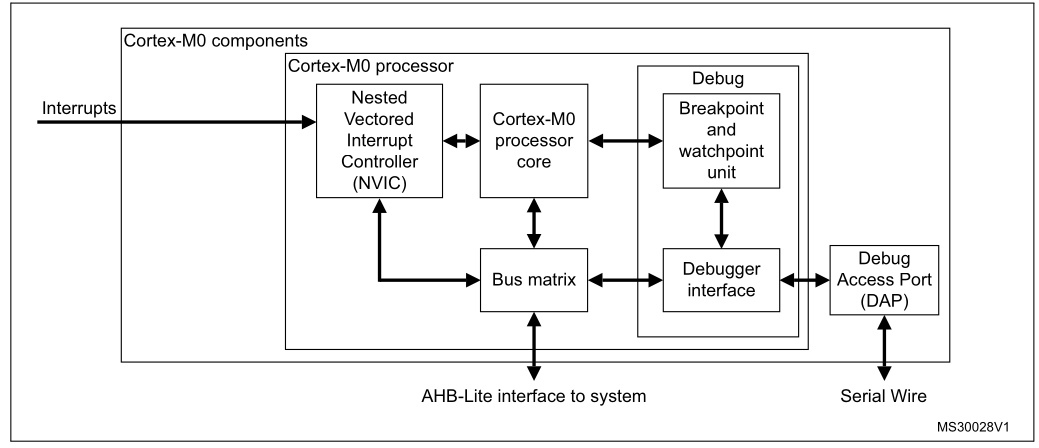
\includegraphics[width=1\linewidth]{cortex}}
    \caption{Реализация ядра Cortex-M0}
\end{figure}

\subsection{Memory map}
Для того чтобы взаимодействовать с какой-либо периферией, необходимо знать адреса регистров, отвечающих за нее. За этим
обращаемся к Memory map:

\begin{figure}[H]
    \center{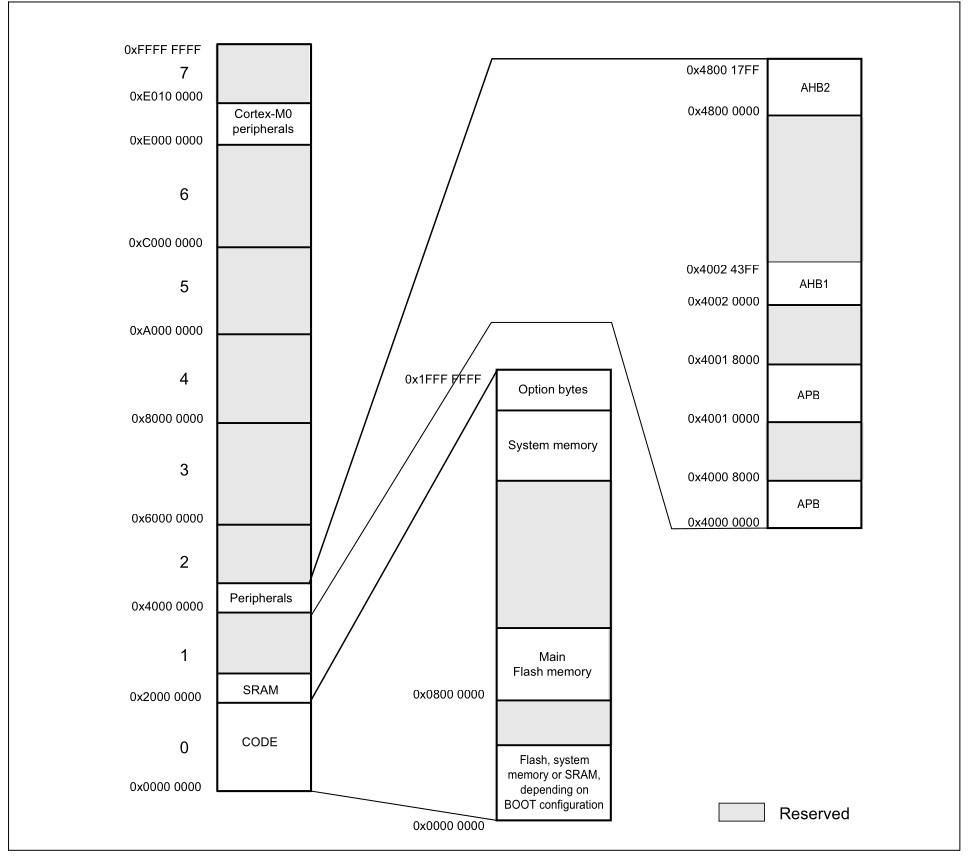
\includegraphics[width=1\linewidth]{memory_map}}
    \caption{Карта памяти и адреса регистров}
\end{figure}

В дальшейшем процессе работы нас будет интересовать работа таймеров. Из карты памяти видно, что за периферию отвечают шины 
AHB(1/2) и APB. Тактирование таймеров будет включаться от шины APB(в дальнейшем обозначается APB1).

Помимо таймеров из периферийных устройств платы так же задействовался диод (вообще говоря, на плате он не один, но
использовать какой-либо, кроме приведенного ниже, не получится). Для того чтобы понять, что он из себя представляет, обратимся
к User Manual \cite{user}:

\begin{figure}[H]
    \center{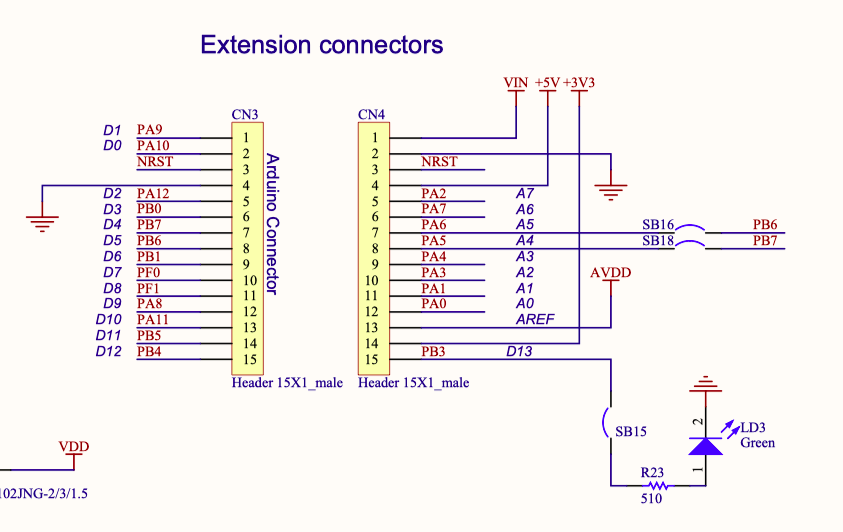
\includegraphics[width=0.8\linewidth]{schema}}
    \caption{Схема пинов и их подключений}
\end{figure}

На данной части схемы видно, что диод находится в правом нижнем углу. Рядом с ним есть подпись LD3 и слово Green. 
Из схемы там же видно что, данный диод подключен к третьему пину порта B (PB3). Соответственно, чтобы включить диод,
нужно будет подать тактирование на этот порт, и настроить нужный пин на вывод.

\subsection{Таймеры}
В работе было задействовано два таймера: TIM2 и TIM3. Это таймеры общего назначения. Они тактируются от шины APB1, 
настроенной на частоту 48 МГц. Для таймеров мы хотим задать периоды в $0.3$ и $0.6$ секунд соответственно.
Опишем вкратце работу таймеров.

\begin{figure}[H]
\centering
    \center{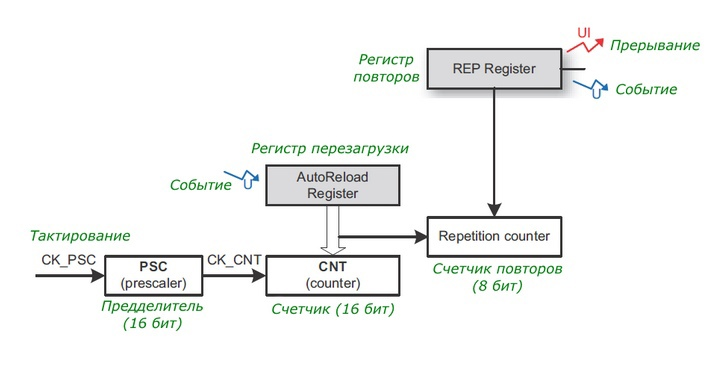
\includegraphics[width=0.7\linewidth]{timers_work}}
    \caption{Принцип работы таймеров}
\end{figure}

Отсчет импульсов или времени происходит на 16-ти разрядном счетчике CNT. Когда код счетчика достигает значения регистра 
перезагрузки, счетчик сбрасывается в 0. Таким образом, счетчик считает по циклу от 0 до значения регистра перезагрузки.
Частота сигнала тактирования таймера может быть уменьшена с помощью 16-ти разрядного предделителя PSC.

Перезагрузка счетчика формирует событие (прерывание). Частота его появления также может быть уменьшена счетчиком повторов (8 разрядов). 
Коэффициент деления задается в регистре повторов.

В качестве режима счетчика сигналов выберем прямой, при котором  содержимое счетчика с каждым импульсом тактирования увеличивается на 1. 
Когда оно достигает значения регистра перезагрузки, то счетчик сбрасывается. Таким образом,таймер считает по циклу от 0 до значения перезагрузки. 

Предделитель делит частоту тактирования таймера, поступающую на основной счетчик.

Таким образом, при заданных выше условиях получаем следующие настройки таймеров:
\begin{figure}[H]
    \begin{subfigure}{.6\linewidth}
        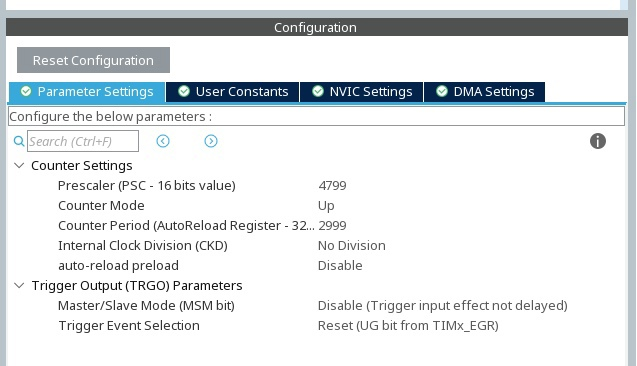
\includegraphics[width=.7\linewidth]{timer2}
        \caption{Второго таймера}
    \end{subfigure}
    \begin{subfigure}{.6\linewidth}
        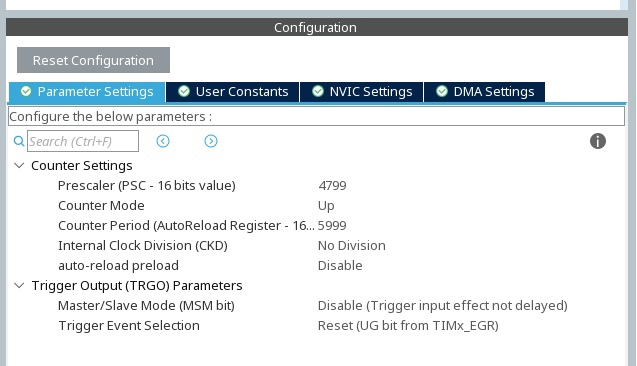
\includegraphics[width=.7\linewidth]{timer3}
        \caption{Третьего таймера}
    \end{subfigure}
    \caption{Настройки таймеров}
\end{figure}

Поскольку шина APB1 тактирует таймеры с частотой $48 \cdot 10^{6}$ Гц, то установив предделитель на значение 4799 (в 
действительности в регистре будет лежать значение на 1 большее), мы получим частоту счетчика $10^4$ Гц. Умножив это 
значение на период счетчика, выставленный в настройках (для второго таймера 2999, для третьего 5999), получим соответственно
$\frac{3000}{10000} = 0.3$ секунды и $\frac{6000}{10000} = 0.6$ секунды. Счетчик повторов устанавливать не будем.
\newpage

\section{Результаты работы}
\subsection{Основная работа}
Стандартный ввод / вывод реализовывался через интерфейс UART(скорость передачи данных $115200$ бод, бит четности четный,
7 битов данных, 1 стоп-бит). Соединение Serial, виртуальный порт -- COM3. Подключаться лучше через приложение Kitty/Putty.
В зависимости от ввода символа доступны следующие возможности:
\begin{enumerate}
\item '1' -- включить диод(при повторном нажатии -- выключить)
\item '0' -- выключить диод
\item '2' -- начать мигание с коротким периодом (10 раз)
\item '3' -- начать мигание с длинным периодом (10 раз)
\end{enumerate}

При срабатывании reset прерывания в терминал выводится следующее меню:
\begin{figure}[H]
    \centering
        \center{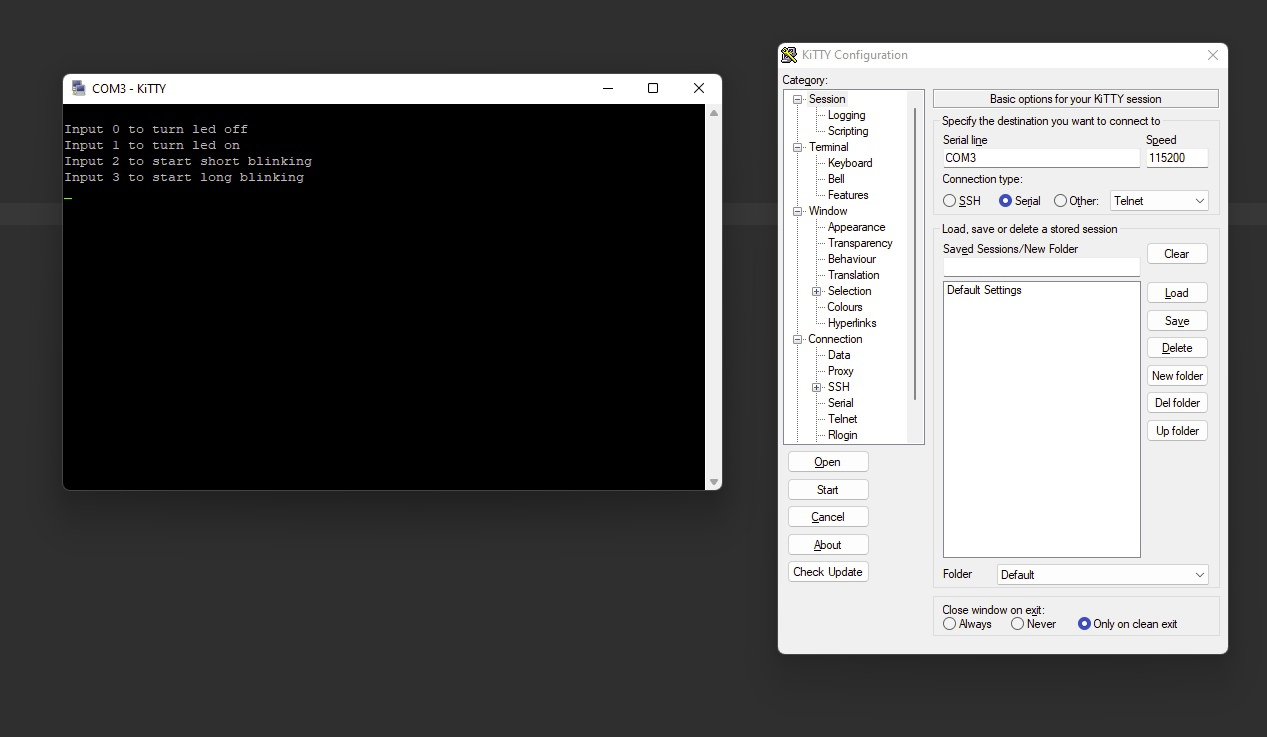
\includegraphics[width=1\linewidth]{menu}}
        \caption{Вывод меню при reset прерывании}
\end{figure}

В работе использовался STM32CubeIDE. Данная среда разработки позволяет настроить конфигурацию, написать программу и 
прошить ее для STM32 контроллера.

\subsection{Дополнительная работа}
Помимо основной задачи так же было реализовано взаимодействие с матрицей кнопок. При работе с ней доступны следющие действия:
\begin{enumerate}
    \item Кнопка '1' -- включить короткое мигание
    \item Кнопка '2' -- включить длинное мигание
    \item Кнопка '3' -- отправить в терминал сообщение о нажатии кнопки 3
    \item Кнопка '4' -- включить выключить диод
\end{enumerate}
Пример срабатывания третьей кнопки можно увидеть ниже:
\begin{figure}[H]
    \centering
        \center{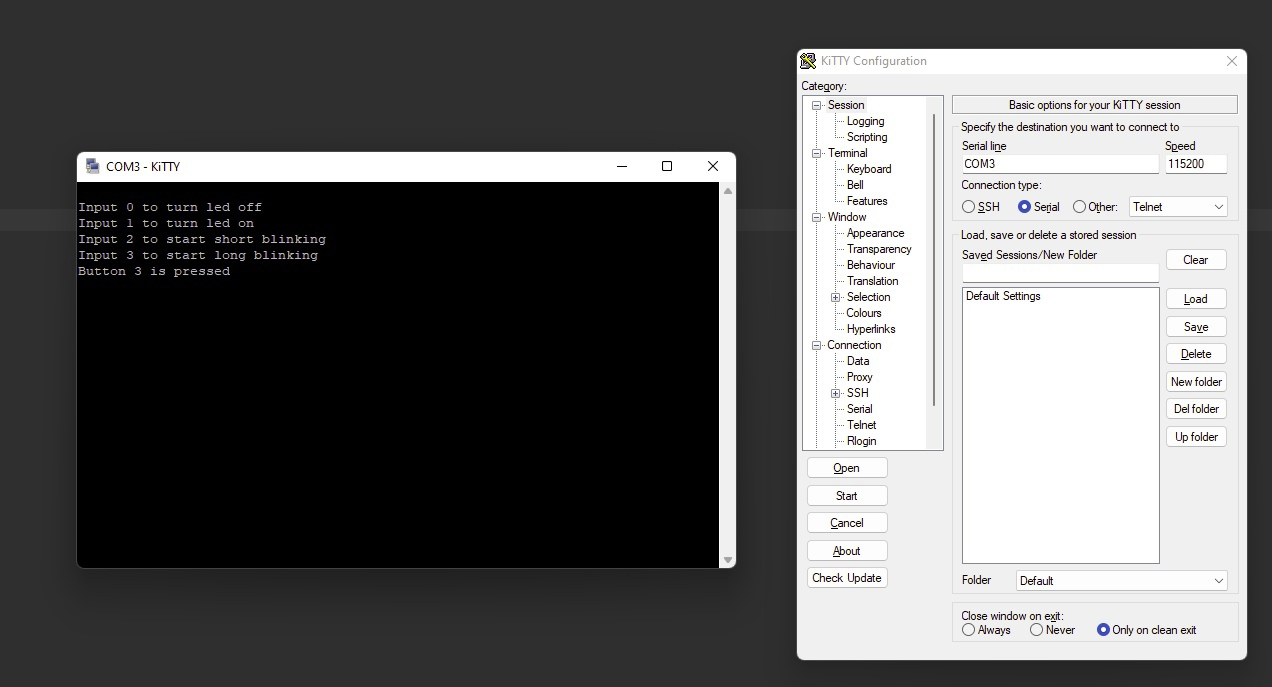
\includegraphics[width=1\linewidth]{button3}}
        \caption{Вывод меню при reset прерывании}
\end{figure}


Для этой задачи были использованы прерывания EXTI, на вырабатывание которых были настроены пины PB7 и PB0. 
\newpage

\section{Итоги}
В ходе работы была изучена работа микроконтроллера STM32, проведены базовые опреации по взаимодействию
между ним и компьютером посредством работы интерфейса UART, а так же рассмотрены и написаны некоторые прерывания,
такие как прерывание таймеров и прерывания, генерируемые EXTI (контроллером внешних прерываний). Так же 
была освоена работа с STM32CubeIDE.

Проект для просмотра доступен по ссылке: 

\url{https://gitlab.com/iliyvas/mps2022/-/tree/kosenko_coursework/Coursework/kosenko}

\begin{thebibliography}{}
\bibitem{prog}
STM32F0xxx Cortex-M0 Programming Manual 
// URL: \url{https://www.st.com/resource/en/programming_manual/pm0215-stm32f0xxx-cortexm0-programming-manual-stmicroelectronics.pdf}
\bibitem{user}
STM32 Nucleo-32 User Manual
// URL: \url{https://www.st.com/resource/en/user_manual/um1956-stm32-nucleo32-boards-mb1180-stmicroelectronics.pdf}
\end{thebibliography}

\end{document}